\chapter{Kísérlet}\label{chap:experiment}

Ebben a fejezetben a kísérleti összeállítás kerül bemutatásra. A motor összeállítás és a mérési eszközök 
részletes dokumentációja után az alkalmazott mérési és vezérlési módszerek sajátosságainak bemutatása 
következik. Ezután szabályozó viselkedésének elemzésére kerül sor az előző fejezetekben bemutatott modellel 
összehasonlítva.

\section{Mérési összeállítás}
A mérésekhez felhasznált egyenáramú motor egy maxon összeállítás része. Az összeállítás egy 
kis teljesítményű DC motorból, egy bolygókerekes hajtóműből és egy enkóderből áll. A motor paraméterei
az \ref{fig:motor_datasheet}. ábrán szereplő adatlapon találhatóak. A hajtómű és az enkóder leírása pedig 
a \ref{fig:gearhead_datasheet}. és \ref{fig:encoder_datasheet}. ábrákon láthatóak. A gravitáció hatásának 
kiküszöbölésére a mérésekhez a motort álló helyzetben kellett rögzíteni. Ehhez készült egy 3D nyomtatott 
műanyag keret, ami a hajtóműhöz csatlakozik. A teljes összeállítás az \ref{fig:setup_experiment}. ábrán 
látható. 
\begin{figure}[H]
    \begin{center}
    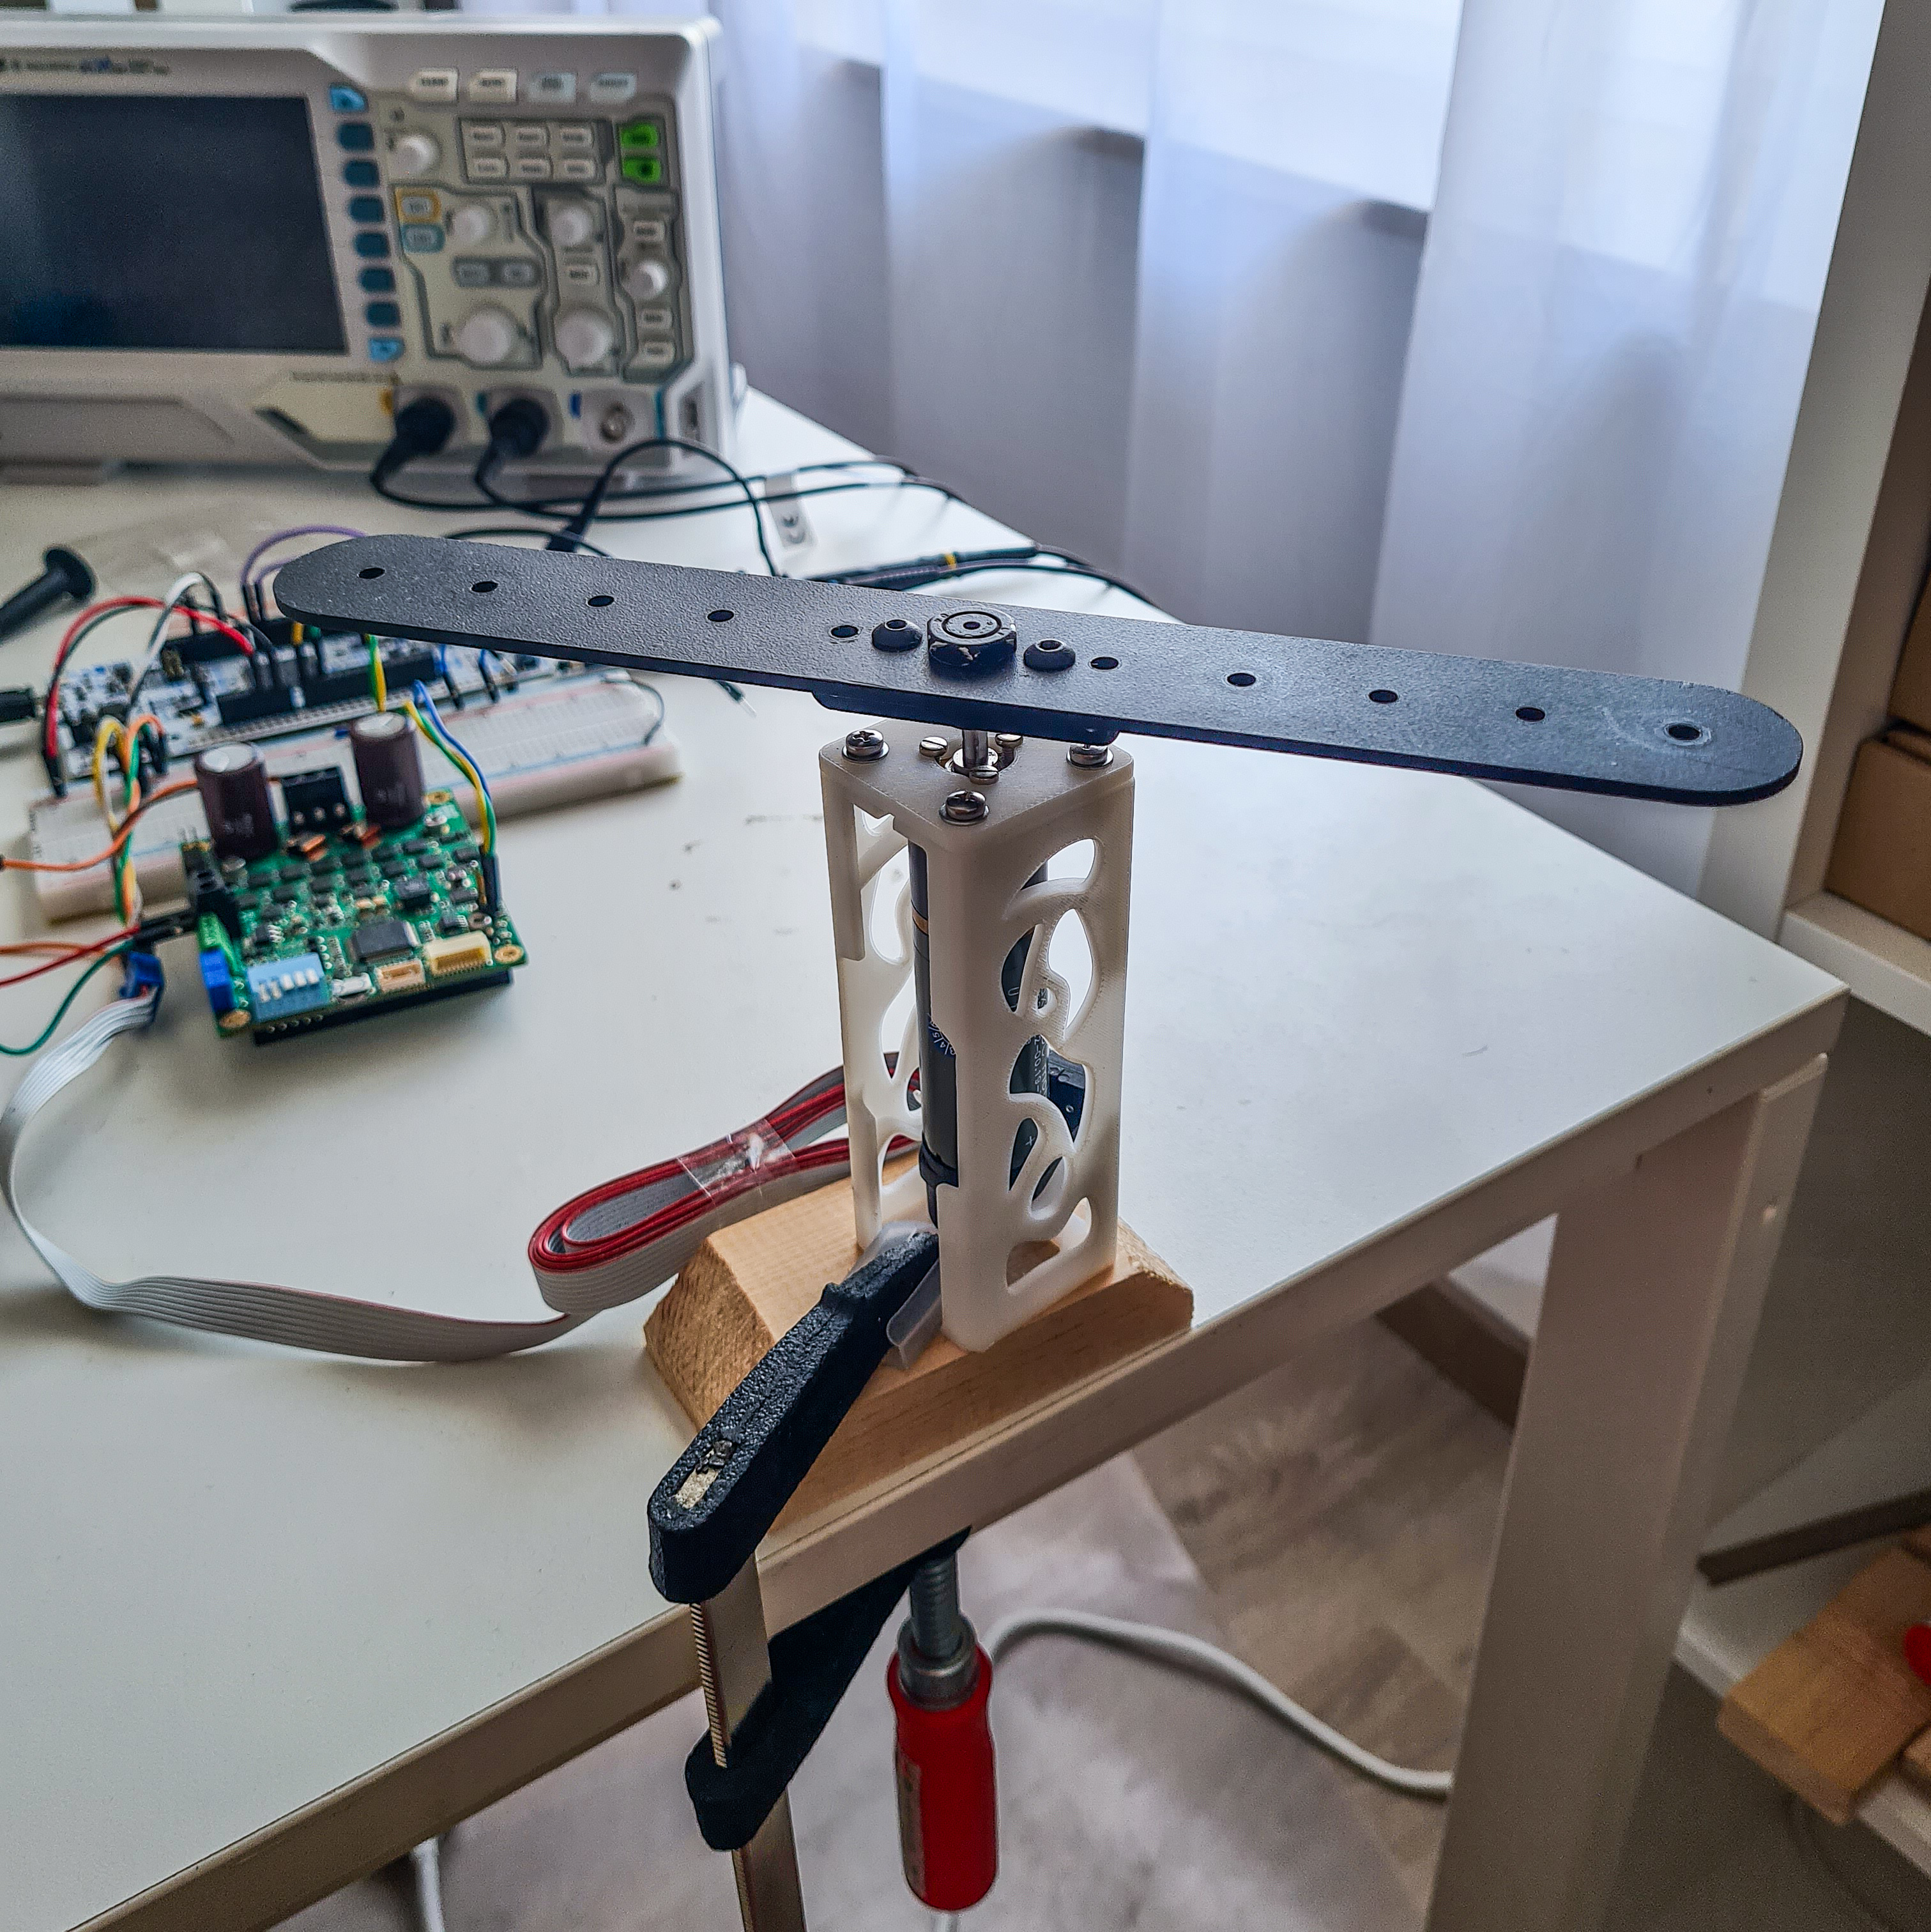
\includegraphics[width=14cm]{images/setup_experiment.jpg}
    \caption{Mérési összeállítás}\label{fig:setup_experiment}
    \end{center}
\end{figure}
A motorvezérlő egy SOLO UNO V2 32A típúsú univerzális vezérlő egység, mely egyenáramú kefés, kefe 
nélküli valamint PMSM és váltakozó áramú indukciós motorok vezérlésére is alkalmas 800W-ig. 
A kimenet változtatható frekvenciájú PWM jel. A kimeneti PWM vezérlő jel frekvenciája elméletben 80kHz-ig 
növelhető. A valóságban 75kHz-es beállítás felett automatikusan visszaugrott a frekvencia 20kHz-re, így 
a kísérletek során 75kHz volt a beállított frekvencia. CANopen és egy egyedi UART 
protokollon keresztül lehet kommunikálni az eszközzel. A kísérletek során a második opció lett alkalmazva.

% Alacsony induktivitású motoroknál, amilyen a kísérletben is felhasznált maxon motor, 
% a vezérlő jel átlagos amplitúdója és a motor nyomatéka között nem feltétlenül van lineáris kapcsolat. 
% Mivel ez egy alapvető feltétele a szabályozó alkalmazhatóságának, most ennek a jelenségnek a 
% részletesebb elemzése következik. A második fejezetben szereplő 
% \eqref{eq:rotor_dynamics} és \eqref{eq:armature_circuit} egyenletek alapján \dots

A szabályozó futtatását egy NUCLEO-F439ZI STMicrocontrollers fejlesztői panel végzi.
Alapvető feladatai:
\begin{itemize}
    \item Az inkrementális enkóder jelének olvasása a beépített számláló és időzítő periférián keresztül
    \item A szabályozó belső állapotának frissítése pontosan meghatározott időközönként.
    \item A szabályozó kimeneti referencia jelének továbbítása a motorvezérlőnek az előírt időkésés figyelembe vételével.
    \item A mérés állapotának felvétele és továbbítása a számítógép felé.
\end{itemize}
A szoftver egyszerűsített vázlata az \ref{fig:block_diagram_control_software}. ábrán látható. 
\begin{figure}[H]
    \begin{center}
    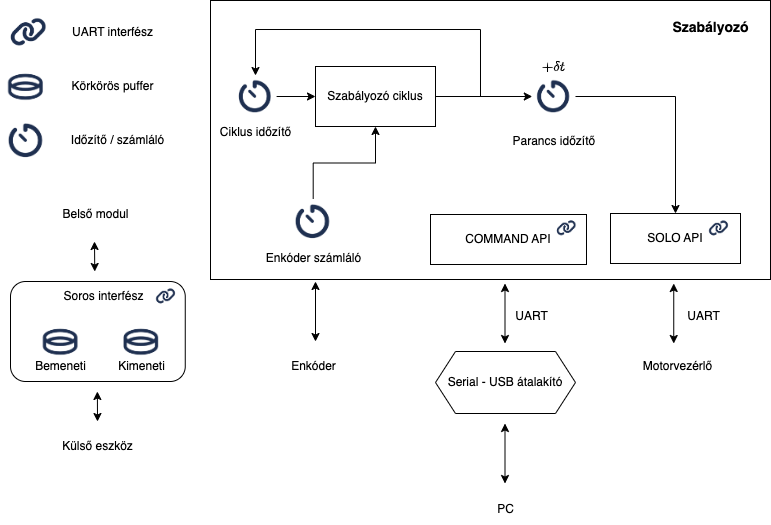
\includegraphics[width=14cm]{images/impedance_controler_software_diagram.png}
    \caption{Szabályozó szoftveres implementációjának egyszerűsített vázlata}\label{fig:block_diagram_control_software}
    \end{center}
\end{figure}
A szabályozó szoftvere egy C-ben írt program, mely az STMicrocontrollers STM32CubeIDE nevezetű 
fejlesztői környezetében készült. Minden időzítéssel kapcsolatos feladatot a beépített perifériák 
látnak el. A szabályozó ciklusa az adott méréshez előre meghatározott ciklusidő / időkésés figyelembe 
vételével periodikusan fut. Az implmentáció a \ref{chap:time_delay_stability}. fejezetben bemutatott 
digitalizált szabályozót követi. Mivel a motorvezérlőnek elküldött parancs meghatározásához szuukséges idő 
lényegesen rövidebb a méréseknél használt ciklusidőknél, egy külön idjozítő felel a parancsok 
megfelelő késleltetéséért. A soros kommunikációhoz szükséges műveleteket soros interfész modulok 
végzik el. Minden interfész modul két körkörös pufferrel rendelkezik. Az egyik a kimenő, a másik puffer 
a válasz üzeneteket tárolja. A pufferek és a UART perifériák közötti adatátvitelt a beépített DMA vezérlők 
valósítják meg. A mérés konfigurálása, nyomonkövetése, és az eredmények visszaküldése a számítógépre 
egy egyszerű protokoll segítségével történik. A protokoll felépítését a \ref{fig:measurement_protocol}. ábra 
mutatja. 
\begin{figure}[H]
    \begin{center}
    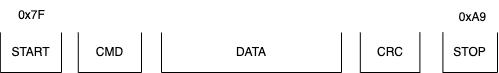
\includegraphics[width=14cm]{images/impedance_controler_software_measurement_protocol.png}
    \caption{A szabályozó kommunikációs protokollja}\label{fig:measurement_protocol}
    \end{center}
\end{figure}
A START, CMD és STOP egy byte hosszúak. A DATA mező fix hosszúságú, legtöbb esetben 4 byte, de a CMD mezőtől függ.
A CMD mező kódolja a parancs típusát. A CRC mező a CMD és DATA mezők alapján számított 8 bites CRC, a kommunikációs 
hibákból eredő félrekonfiguráció esélyének csökkentéséért felel. 

A mérésekhez felhasznált egyéb eszközök a \ref{tab:measurement_tools}. táblázatban találhatóak.
\begin{table}[H]
    \small\centering
    \caption{További mérési eszközök}\label{tab:measurement_tools}
    \tabcolsep=1pt
    \begin{tabular}{l>{~}l>{~}l>{\quad}rl}
        \toprule
        \multicolumn{1}{c}{Eszköz neve} & \multicolumn{1}{c}{Gyártója} & \multicolumn{1}{c}{Típusa} & \multicolumn{2}{c}{Precizitás} \\ \midrule
        Mérőórás tolómérő & Berger & 020701-0007 & \(\pm\)0.02 & mm \\
        Digitális oszcilloszkóp & Rigol & DS1202Z-E & 200 MHz / 1 & GSa/s \\
        DC laboratóriumi tápegység & UNI-T & UTP3315TFL-II & 0-30V \(\pm\) 10 mV, 0-5A \(\pm\) 1 & mA \\
        Digitális multiméter & MAXWELL & MX-25304 & \(\pm\)0.1 mV - 1 V, \(\pm\) 0.1 \(\mu\)A - 10 & mA \\
        \bottomrule
    \end{tabular}
\end{table}

\section{Paraméter identifikáció}
A szabályozó megfelelő működésének feltétele, hogy rendelkezésre álljanak a motor pontos paraméterei. 
Bár az adatlapokból több szükséges paraméter is kiolvasható, vannak paraméterek, amiket külön kellett 
meghatározni. Ilyen a motorra terhelésként ráhelyezett propeller tehetetlenségi nyomatéka és a viszkózus 
csillapítási tényező. A hajtómű áttétele, a rotor tehetetlenségi nyomatéka és a nyomatékállandó esetében 
az adatlapokban szereplő értékek lettek alkalmazva. A rotor ellenállása és a motorvezérlő motorra adott 
feszültségjelének amplitúdója és a vezérlő parancs közötti viszony külön lettek meghatározva. 

A rotor ellenállásának meghatározásához egy sor állandó feszültség lett kapcsolva a motorra 
lefogott állapotban, és a motor által felvett áram került feljegyzésre. A mért értékek a \ref{tab:resistance_measurement}. 
táblázatban találhatóak. 
\begin{table}[H]
    \small\centering
    \caption{Ellenállás mérés adatok}\label{tab:resistance_measurement}
    \tabcolsep=2pt
    \begin{tabular}{d{-1}>{~}d{-1}>{~}d{1}cl}
        \toprule
        \multicolumn{1}{c}{Kapocsfeszültség [V]} & \multicolumn{1}{c}{Felvett áram [A]} & \multicolumn{3}{c}{Ellenállás [\(\Omega\)]} \\ 
        \multicolumn{1}{c}{(mind \(\pm\) 0.01)} & \multicolumn{1}{c}{(mind \(\pm\) 0.01)} \\
        \midrule
        2.02 & 0.22 & 9.2 & \(\pm\) & 0.4 \\
        2.48 & 0.28 & 8.8 & \(\pm\) & 0.3 \\
        2.64 & 0.29 & 9.1 & \(\pm\) & 0.3 \\
        2.97 & 0.37 & 8.0 & \(\pm\) & 0.2 \\
        2.95 & 0.29 & 10.2 & \(\pm\) & 0.4 \\
        3.26 & 0.37 & 8.8 & \(\pm\) & 0.2 \\
        3.26 & 0.38 & 8.6 & \(\pm\) & 0.2 \\
        3.39 & 0.41 & 8.3 & \(\pm\) & 0.2 \\
        3.46 & 0.39 & 8.9 & \(\pm\) & 0.2 \\
        3.95 & 0.46 & 8.6 & \(\pm\) & 0.19 \\
        4.05 & 0.46 & 8.8 & \(\pm\) & 0.2 \\
        4.24 & 0.51 & 8.3 & \(\pm\) & 0.16 \\
        4.51 & 0.52 & 8.7 & \(\pm\) & 0.17 \\
        4.89 & 0.62 & 7.9 & \(\pm\) & 0.13 \\
        5.08 & 0.65 & 7.8 & \(\pm\) & 0.12 \\
        \midrule
        & \multicolumn{1}{r}{\(\bar R = \)} & 8.7 & \(\pm\) & 0.15 \\
        \bottomrule
    \end{tabular}
\end{table}
A mérések alapján kapott átlag bizonytalansága az egyes minták szórásából számított 
standard hiba. Ez az érték szignifikánsan eltér az adatlapban szereplő értéktől. A 
későbbi mérések alapján az adatlapban szereplő érték nem lett felhasználva.

A propeller tehetetlenségi nyomatéka lengési idők mérése alapján lett meghatározva. Egy 
adott ponton felfüggesztett merev test lengési periódusát, mely a gravitáció hatására 
szabadon leng egy síkban, a következő összefüggés írja le
\begin{equation}
    t_l = 2\pi\sqrt{\frac{I_\RM P}{mgd}},
\end{equation}
ahol \(I_\RM{P}\) a test másodrendű nyomatéka, \(m\) a tömege, \(g\) a gravitációs állandó, 
és \(d\) a felfüggesztési pont és a test tömegözéppontja közötti távolság. 
Kifejezve a tehetetlenségi nyomatékot 
\begin{equation}
    I_\RM{P} = \frac{mgd}{4\pi^2}t^2_l,
\end{equation}
A mérési összeállítást szemlélteti a \ref{fig:propeller_pendulum}. ábra. Az 
előbbi formula relatíve kis kilengés esetén alkalmazható, így nagyjából 
10° volt a kezdeti kilengés.
\begin{figure}[H]
    \begin{center}
    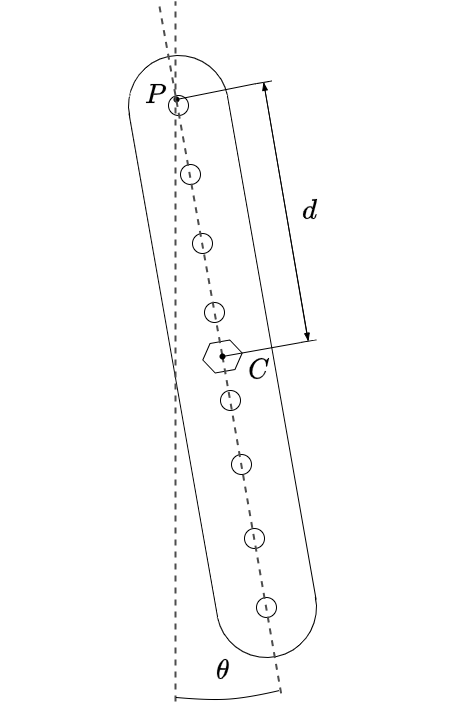
\includegraphics[height=12cm]{images/impedance_control_propeller.png}
    \caption{Felfüggesztett terhelés tehetetlenségi nyomaték méréshez}\label{fig:propeller_pendulum}
    \end{center}
\end{figure}
Minden mérés során harminc oda-vissza 
lengés ideje lett lemérve. Az eredmények a \ref{tab:propeller_period_measurement}. táblázatban találhatóak. A számított 
átlag a standard hibával együtt az utolsó sorban található. Az átlag már az egy periódusra számított 
időt mutatja.
\begin{table}[H]
    \small\centering
    \caption{Terhelés lengési idő mérési adatok}\label{tab:propeller_period_measurement}
    \tabcolsep=2pt
    \begin{tabular}{rd{-1}}
        \toprule
        \multicolumn{2}{c}{30 lengés periódus ideje [s]} \\ 
        \multicolumn{2}{c}{\(t_{30}\)} \\
        \midrule
        & 22.35 \\
        & 22.20 \\
        & 22.27 \\
        & 22.26 \\
        & 22.19 \\
        \midrule
        \multicolumn{1}{r}{\(\bar t_\RM l = \)} & \multicolumn{1}{c}{0.742 \(\pm\) 0.001} \\
        \bottomrule
    \end{tabular}
\end{table}
A későbbi mérésekhez a formulában szereplő felfüggesztéshez viszonyított tehetetlenségi 
nyomatékkal elleben a tömegközéppontra számított tehetetlenségi nyomatékra van szükség. 
A Steiner-tétel alapján
\begin{equation}
    I_\RM{cm} = I_\RM{P} - md^2,
\end{equation}
A számításhoz szükséges összes paramétert a \ref{tab:propeller_measurement_summary}.
táblázat tartalmazza.
\begin{table}[H]
    \small\centering
    \caption{Terhelés tehetetlenségi nyomaték számítás adatok}\label{tab:propeller_measurement_summary}
    \tabcolsep=2pt
    \begin{tabular}{ccc}
        \toprule
        \multicolumn{1}{c}{Periódusidő [s]} & \multicolumn{1}{c}{Felfüggesztés távolsága [mm]} & \multicolumn{1}{c}{Propeller tömege [g]}\\ 
        \multicolumn{1}{c}{\(t_\RM l\)} & \multicolumn{1}{c}{\(d\)} & \multicolumn{1}{c}{\(m\)} \\
        \midrule
        0.742 \(\pm\) 0.001 & 110 \(\pm\) 1 & 43 \(\pm\) 1 \\
        \bottomrule
    \end{tabular}
\end{table}
A felfüggesztés és a propeller tömegközéppontja közötti távolság ugyan a \ref{tab:measurement_tools}. 
táblázatban szereplő tolómérővel lett meghatározva, a felfüggesztéshez használt drót rugalmassága miatt 
a felfüggesztési pont számomra nem egy jól definiált pont az eszköz precizitását figyelembe véve. Emiatt 
nagyobb a bizonytalanság ebben a paraméterben.

A gravitációs állandó étéke minden esetben \(g = 9.80 \frac{m}{s^2}\). További feltételezés, hogy a 
hibaszámítások során bizonytalansága elhanyagolhatónak tekinthető. Ezek alapján a propeller 
tehetetlenségi nyomatéka
\begin{equation}
    I_\RM{cm} = (1.26 \pm 0.05)\times10^{-4}~\RM{kg \cdot m^2}.
\end{equation}

A motorvezérlő linearitásának ellenőrzéséhez és a motorra eső feszültség pontosabb meghatározásához 
a motor kapocsfeszültsége és PWM vezérlő jel kitöltési tényezője is ki lett mérve különböző esetekben.
A mérési eredményeket a \ref{tab:driver_linearity_measurements}. táblázat tartalmazza. A két paraméter közötti kapcsolatot modellező 
egyenes lineáris regresszióval lett meghatározva. Ez az egyenes a mérési pontokkal együtt a \ref{fig:driver_linearity}.
ábrán látható.
\begin{table}[H]
    \small\centering
    \caption{Vezérlő jel és kapocsfeszültség mérések}\label{tab:driver_linearity_measurements}
    \tabcolsep=2pt
    \begin{tabular}{d{-1}>{~}d{-1}}
        \toprule
        \multicolumn{1}{c}{Kitöltési tényező [\%]} & \multicolumn{1}{c}{Kapocsfeszültség [V]} \\ 
        \multicolumn{1}{c}{\(f\) (mind \(\pm 0.1\))} & \multicolumn{1}{c}{\(V_\RM k\) (mind \(\pm 0.01\))} \\
        \midrule
        16.7 & 1.79 \\
        26.7 & 2.99 \\
        36.7 & 4.19 \\
        46.7 & 5.40 \\
        56.7 & 6.61 \\
        66.7 & 7.82 \\
        76.7 & 9.02 \\
        \bottomrule
    \end{tabular}
\end{table}
\begin{figure}[H]
    \begin{center}
    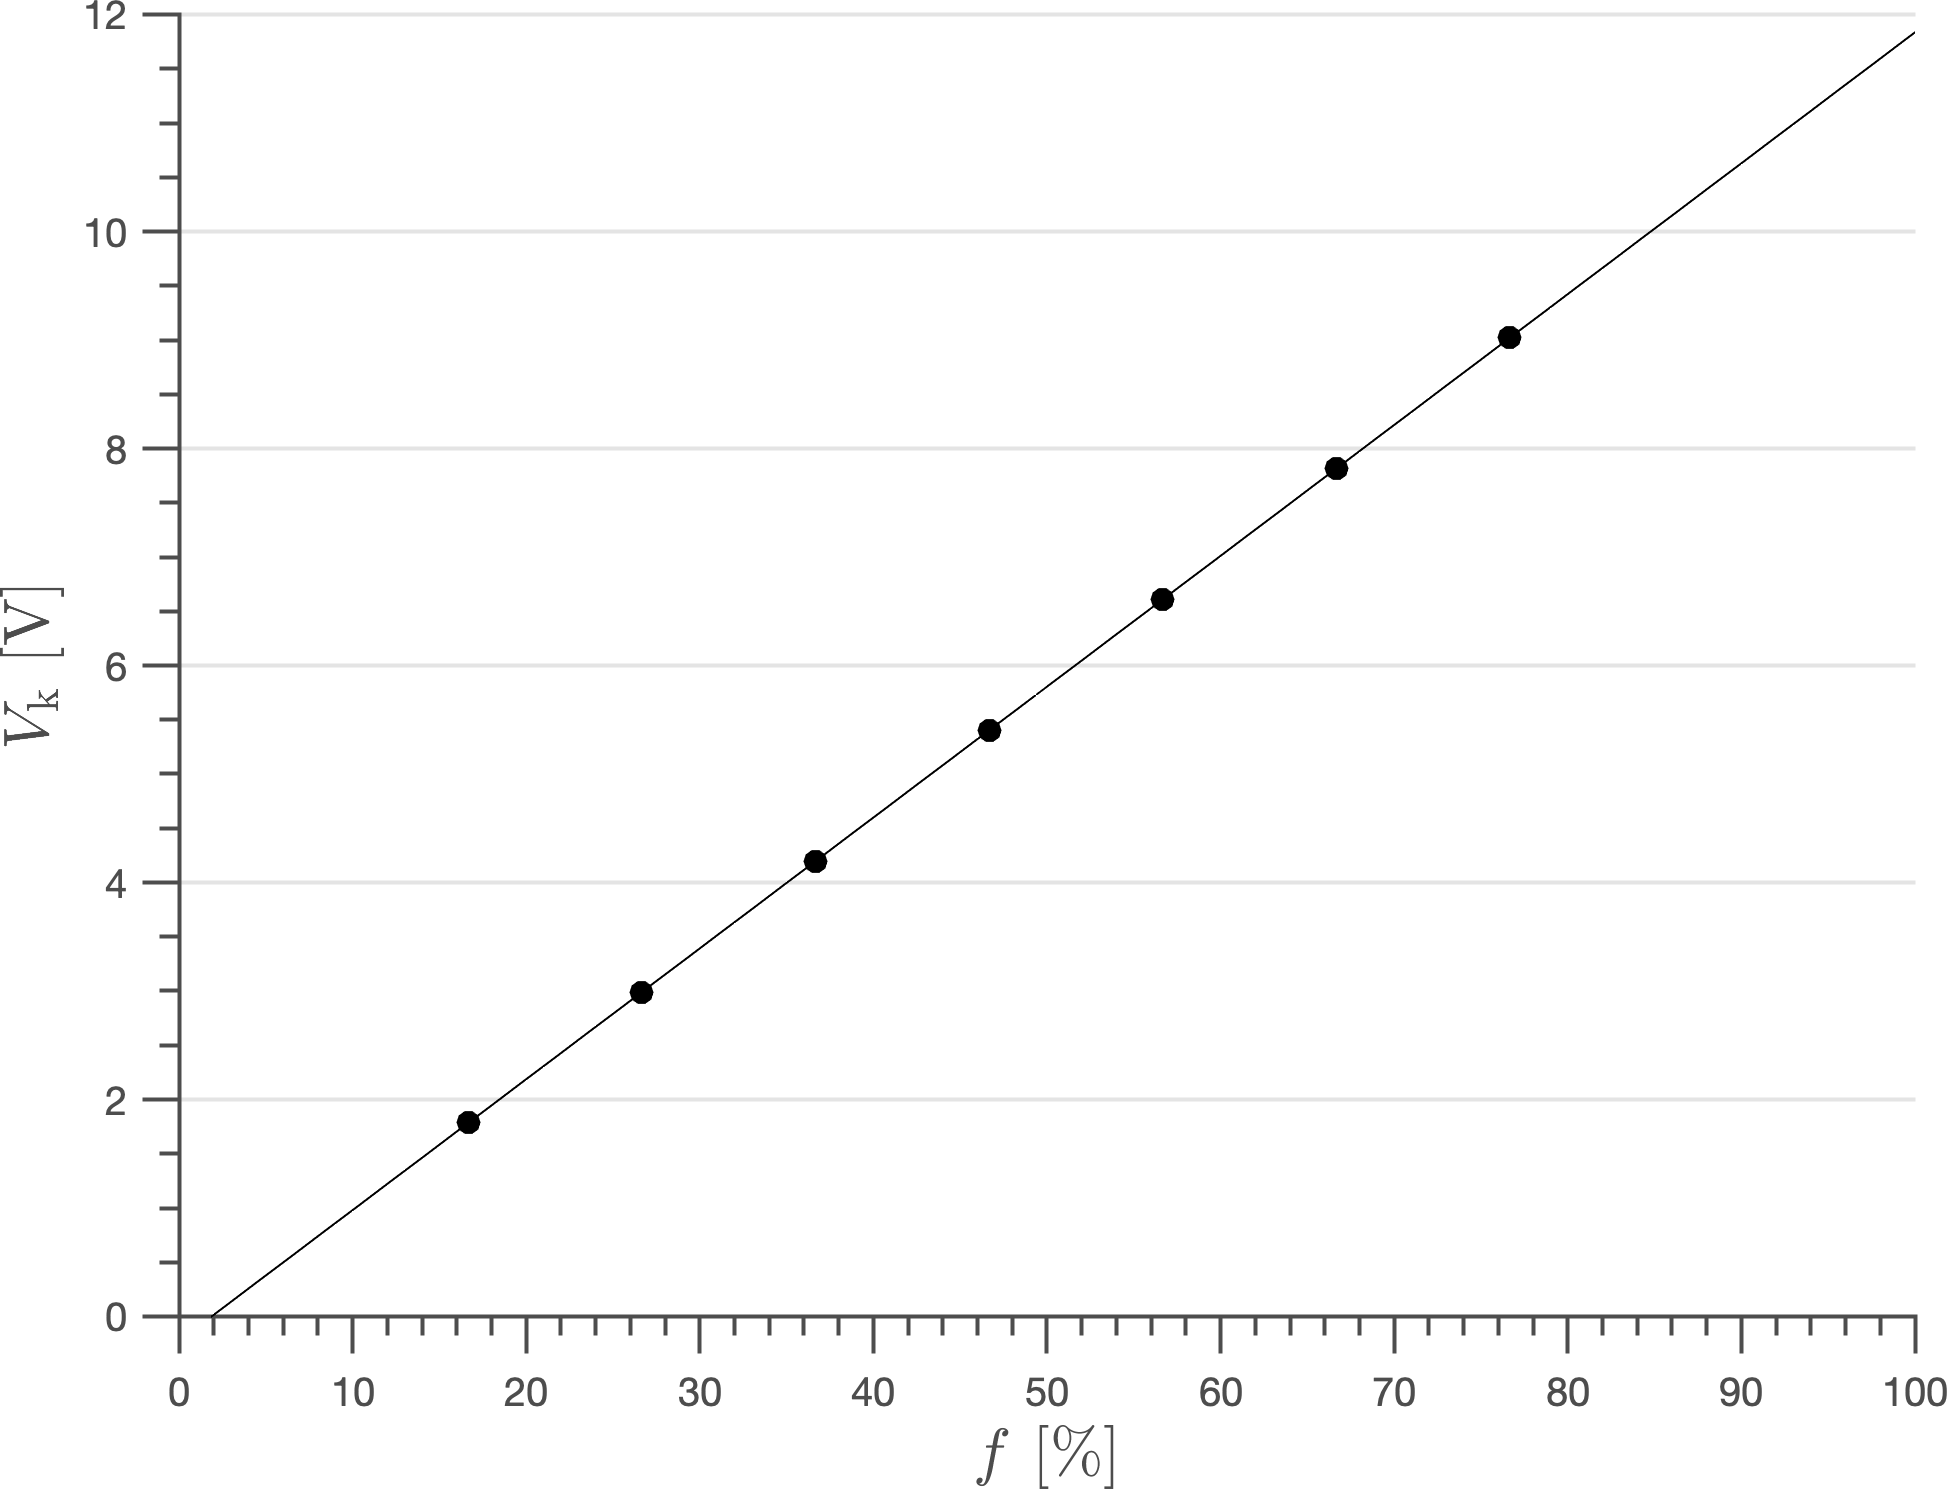
\includegraphics[width=14cm]{images/driver_linearity.png}
    \caption{Motor driver lineáritás vizsgálata}\label{fig:driver_linearity}
    \end{center}
\end{figure}
A hibasávok kis méretük miatt nem lettek ábrázolva. A motorvezérlő kimenetének linearitása 
jól látható.
A maximális feszültség ez alapján kcisit alacsonyabb a motorvezérlőnek bementként adott 
nominális 12V-os feszültségnél. Értéke \(V_\RM{max} = 11.835 \pm 0.005~[\RM V]\).

Az adatlapokban szereplő értékekkel kiegészítve a \eqref{eq:armature_circuit} és \eqref{eq:rotor_dynamics}
egyenletek alapján meghatározható a modell viszkózus csillapítási állandója, ha a motor állandósult 
állapotában mért sebessége is meghatározható. Ennek a mérésnek az eredményeit foglalja össze a \ref{tab:speed_profile}.
táblázat. A lineáris regresszióval illesztett egyenes és a mérési pontok a \ref{fig:speed_profile}. ábrán látható. 
\begin{table}[H]
    \small\centering
    \caption{Motor végsebesség és kapocsfeszültség mérések}\label{tab:speed_profile}
    \tabcolsep=2pt
    \begin{tabular}{d{-1}>{~}d{-1}}
        \toprule
        \multicolumn{1}{c}{Kapocsfeszültség [V]} & \multicolumn{1}{c}{Rotor sebessége [rad/s]} \\ 
        \multicolumn{1}{c}{\(V_\RM k\) (mind \(\pm 0.01\))} & \multicolumn{1}{c}{\(\omega_\RM r\) (mind \(\pm 0.1\))} \\
        \midrule
        1.18 & 36.3 \\
        1.38 & 54.7 \\
        1.58 & 68.1 \\
        1.78 & 79.9 \\
        1.97 & 94.3 \\
        2.17 & 106.6 \\
        2.37 & 120.0 \\
        2.56 & 133.1 \\
        2.76 & 146.5 \\
        2.96 & 160.3 \\
        3.16 & 173.7 \\
        3.35 & 187.6 \\
        3.55 & 199.1 \\
        3.75 & 211.8 \\
        3.94 & 224.7 \\
        4.14 & 237.2 \\
        4.34 & 250.4 \\
        4.54 & 262.4 \\
        4.73 & 274.7 \\
        4.93 & 287.3 \\
        5.13 & 299.7 \\
        5.33 & 311.8 \\
        5.52 & 324.3 \\
        5.72 & 336.4 \\
        5.92 & 349.0 \\
        6.11 & 361.6 \\
        6.31 & 374.1 \\
        6.51 & 386.2 \\
        6.71 & 397.8 \\
        6.90 & 410.0 \\
        7.10 & 420.8 \\
        7.30 & 432.1 \\
        7.50 & 445.3 \\
        7.69 & 456.5 \\
        7.89 & 469.2 \\
        8.09 & 479.9 \\
        8.28 & 491.1 \\
        8.48 & 502.2 \\
        8.68 & 514.1 \\
        8.88 & 526.6 \\
        9.07 & 537.2 \\
        9.27 & 549.2 \\
        9.47 & 560.4 \\
        9.67 & 571.7 \\
        9.86 & 582.9 \\
        \bottomrule
    \end{tabular}
\end{table}
\begin{figure}[H]
    \begin{center}
    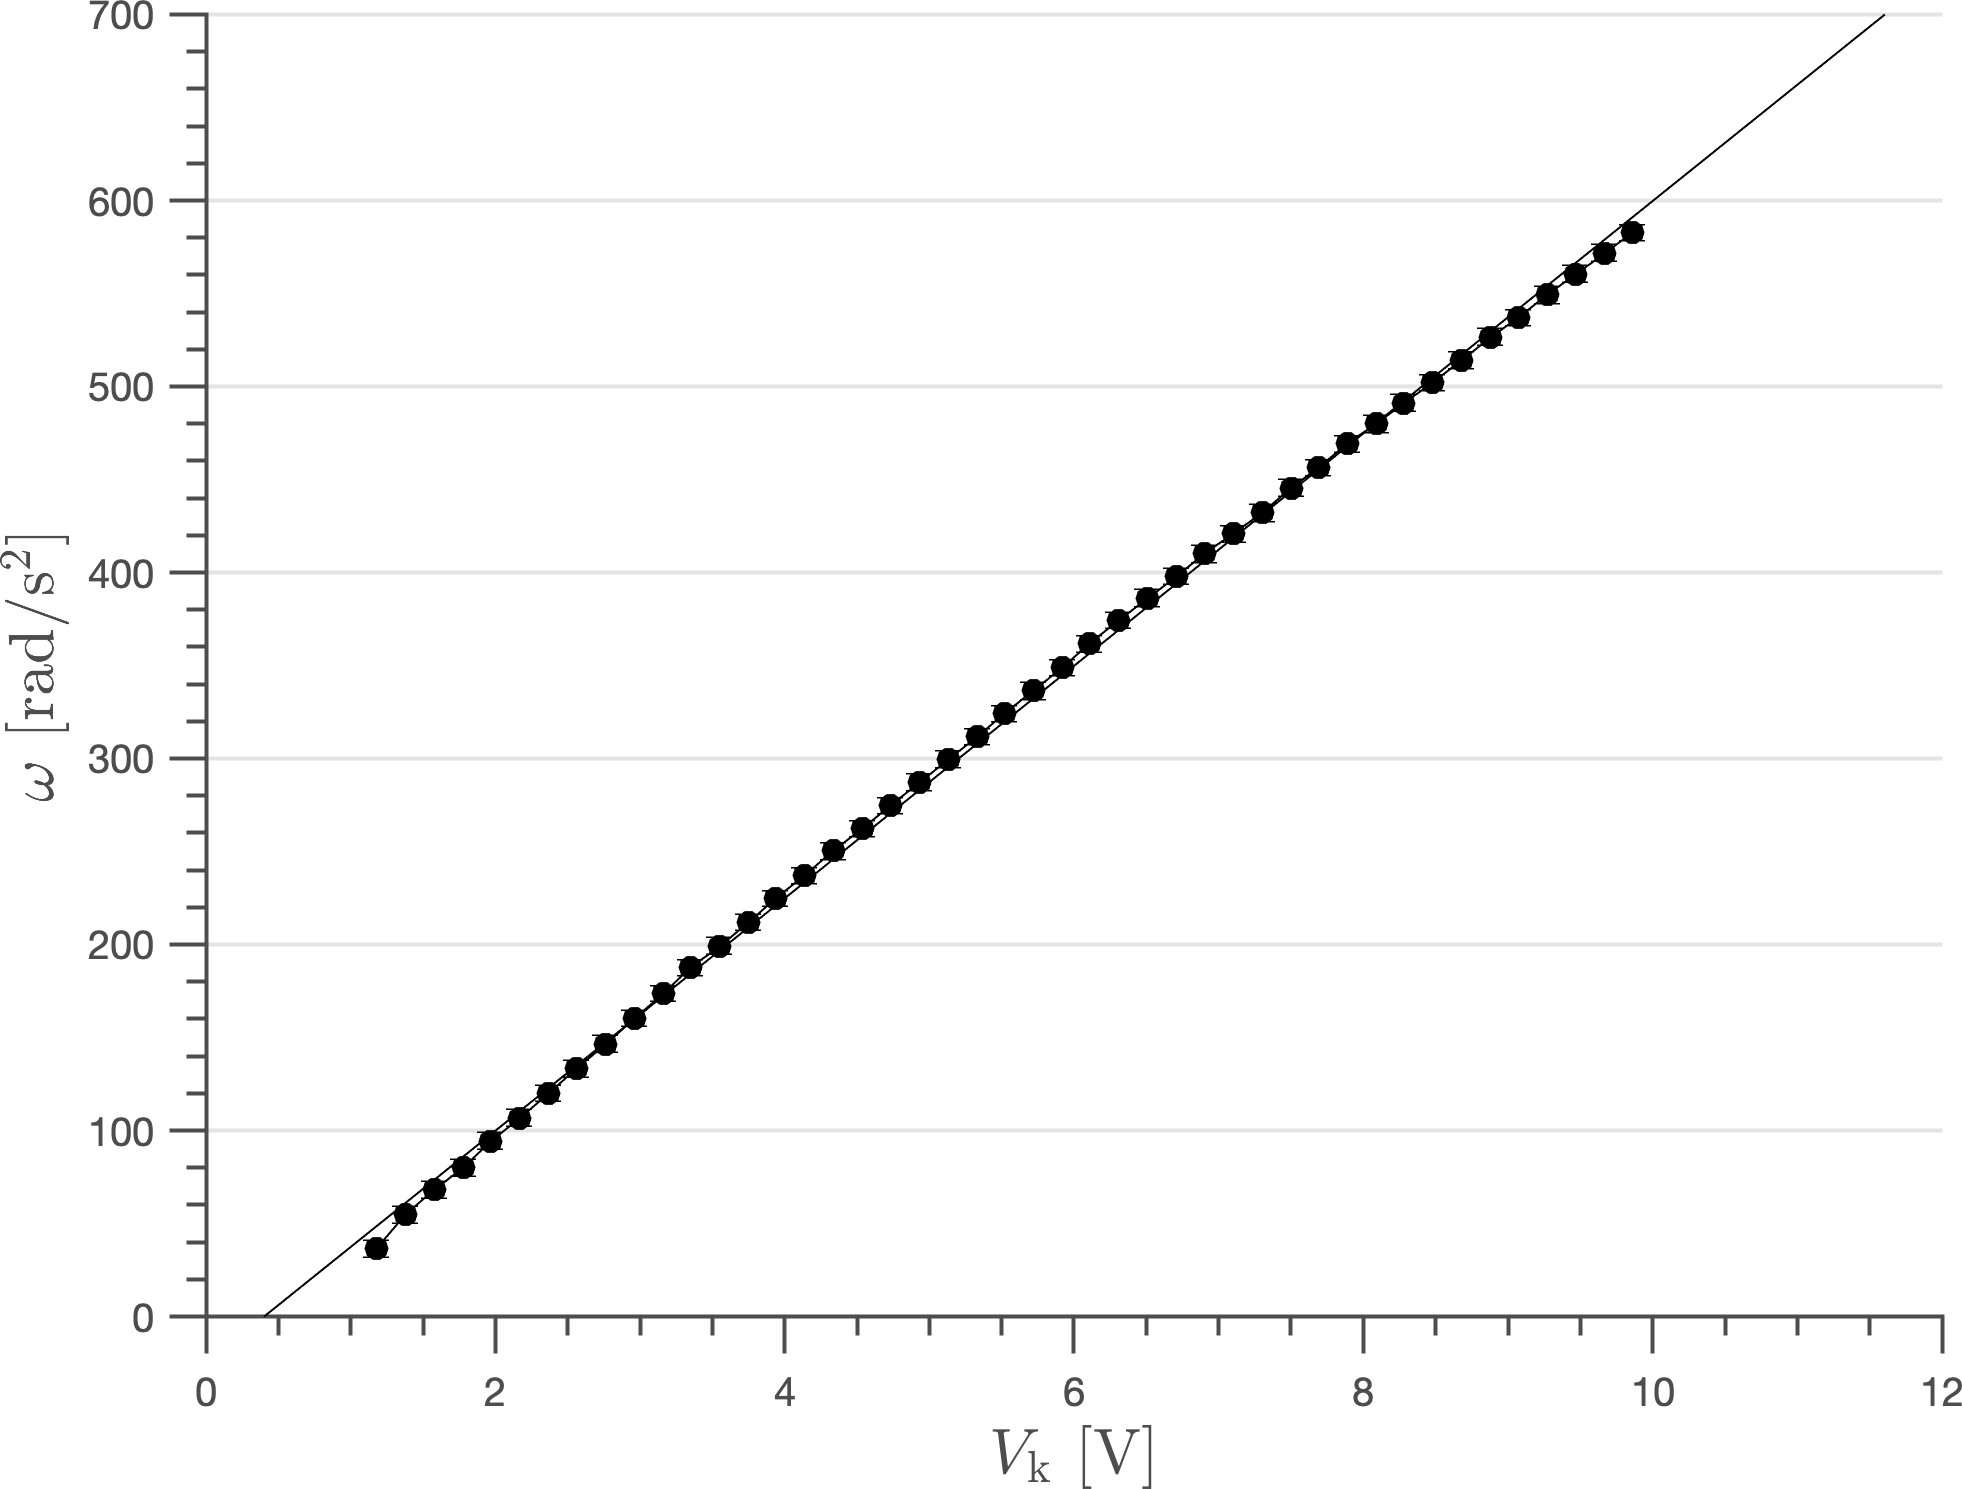
\includegraphics[width=14cm]{images/speed_profile.png}
    \caption{Motor végsebesség és kapocsfeszültség közötti kapcsolat}\label{fig:speed_profile}
    \end{center}
\end{figure}
A viszkózus csillapítási együtthatóra kapott becslés így
\begin{equation}
    B_\RM m = \frac{K_\RM m}{R}\left(\frac{1}{\alpha_\RM s} - K_\RM m\right),
\end{equation}
ahol \(\alpha_s\) az állandósult sebesség és a kapocsfeszültség közötti kapcsolatot 
leíró lineáris regresszióból kapott egyenes meredeksége. Minden paraméter ismert bizonytalanságukkal 
együtt. A végleges becslés
\begin{equation}
    B_\RM m = (1.1 \pm 0.1)\times 10^{-6}~\RM{kg\cdot m^2\cdot s^{-1}}.
\end{equation}

\section{Eredmények}
A motorparaméterek meghatározása után lehetőség nyílt a valós rendszer és a szimuláció összehasonlítására.
Az egységugrásra adott válasz összehasonlítását a szimulált digitális szabályozóval és a beállított impedancia modellel 
az \ref{fig:}. ábra mutatja. Az időkésés \(\tau = 5~\RM{ms}\). Az impedancia modell paraméterei 
\(M_\RM e = 5~\RM{kg \cdot m^2}\), 

A stabilitásvizsgálat eredményeinek ellenőrzéséhez 

\begin{figure}[H]
    \begin{center}
    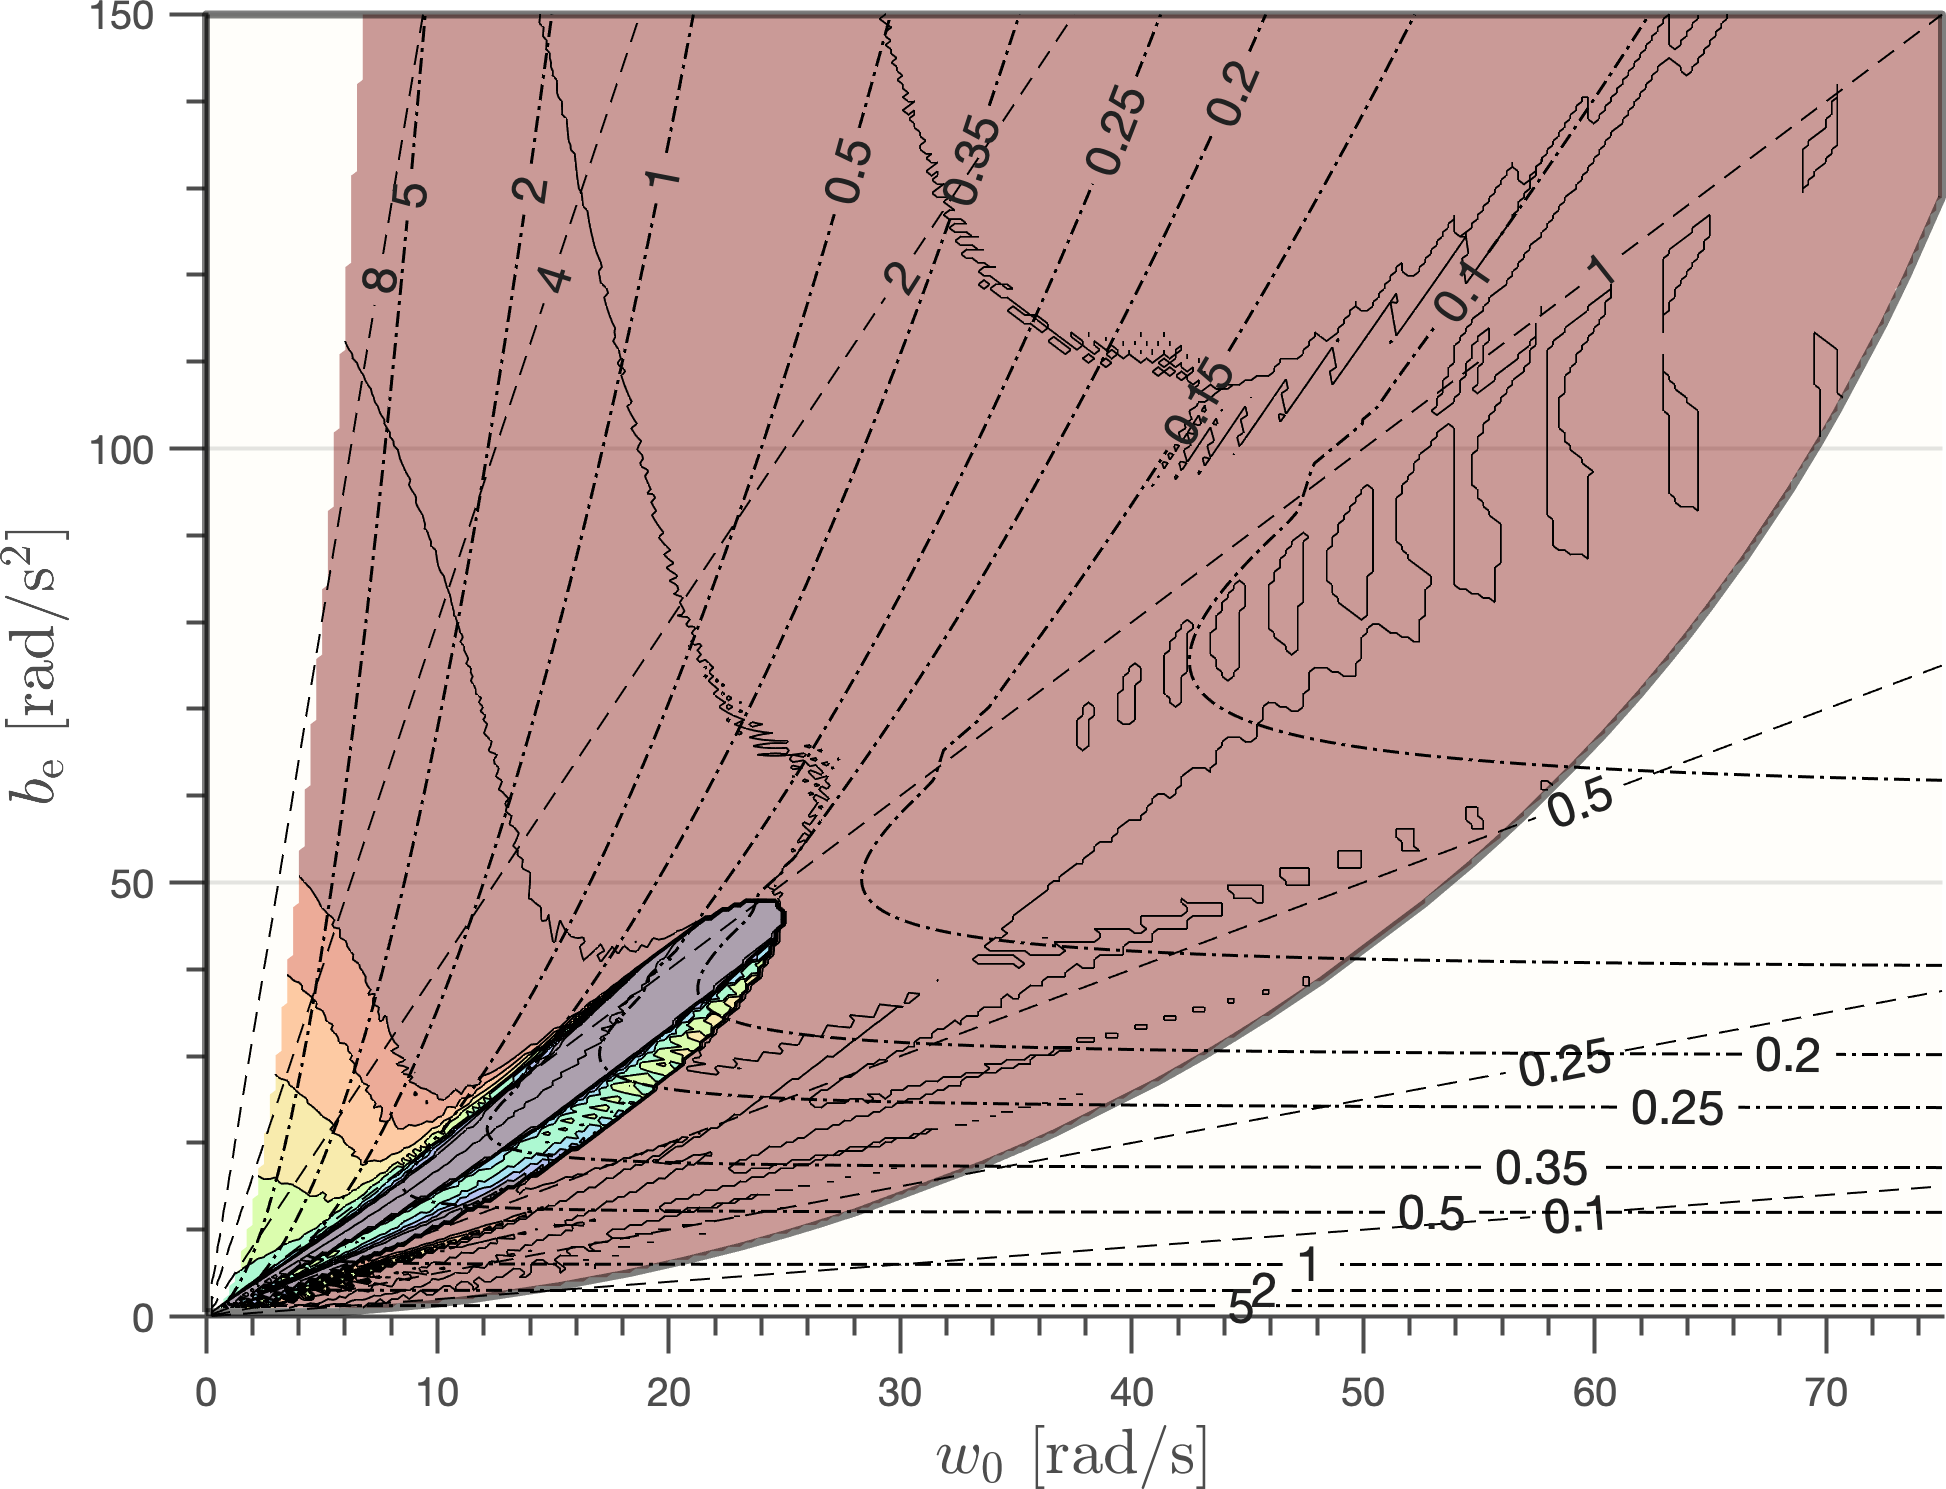
\includegraphics[width=\textwidth]{images/stab_map_001.png}
    \caption{Stabilitástérkép 10ms időkéséssel}\label{fig:stab_map_001}
    \end{center}
\end{figure}

\begin{figure}[H]
    \begin{center}
    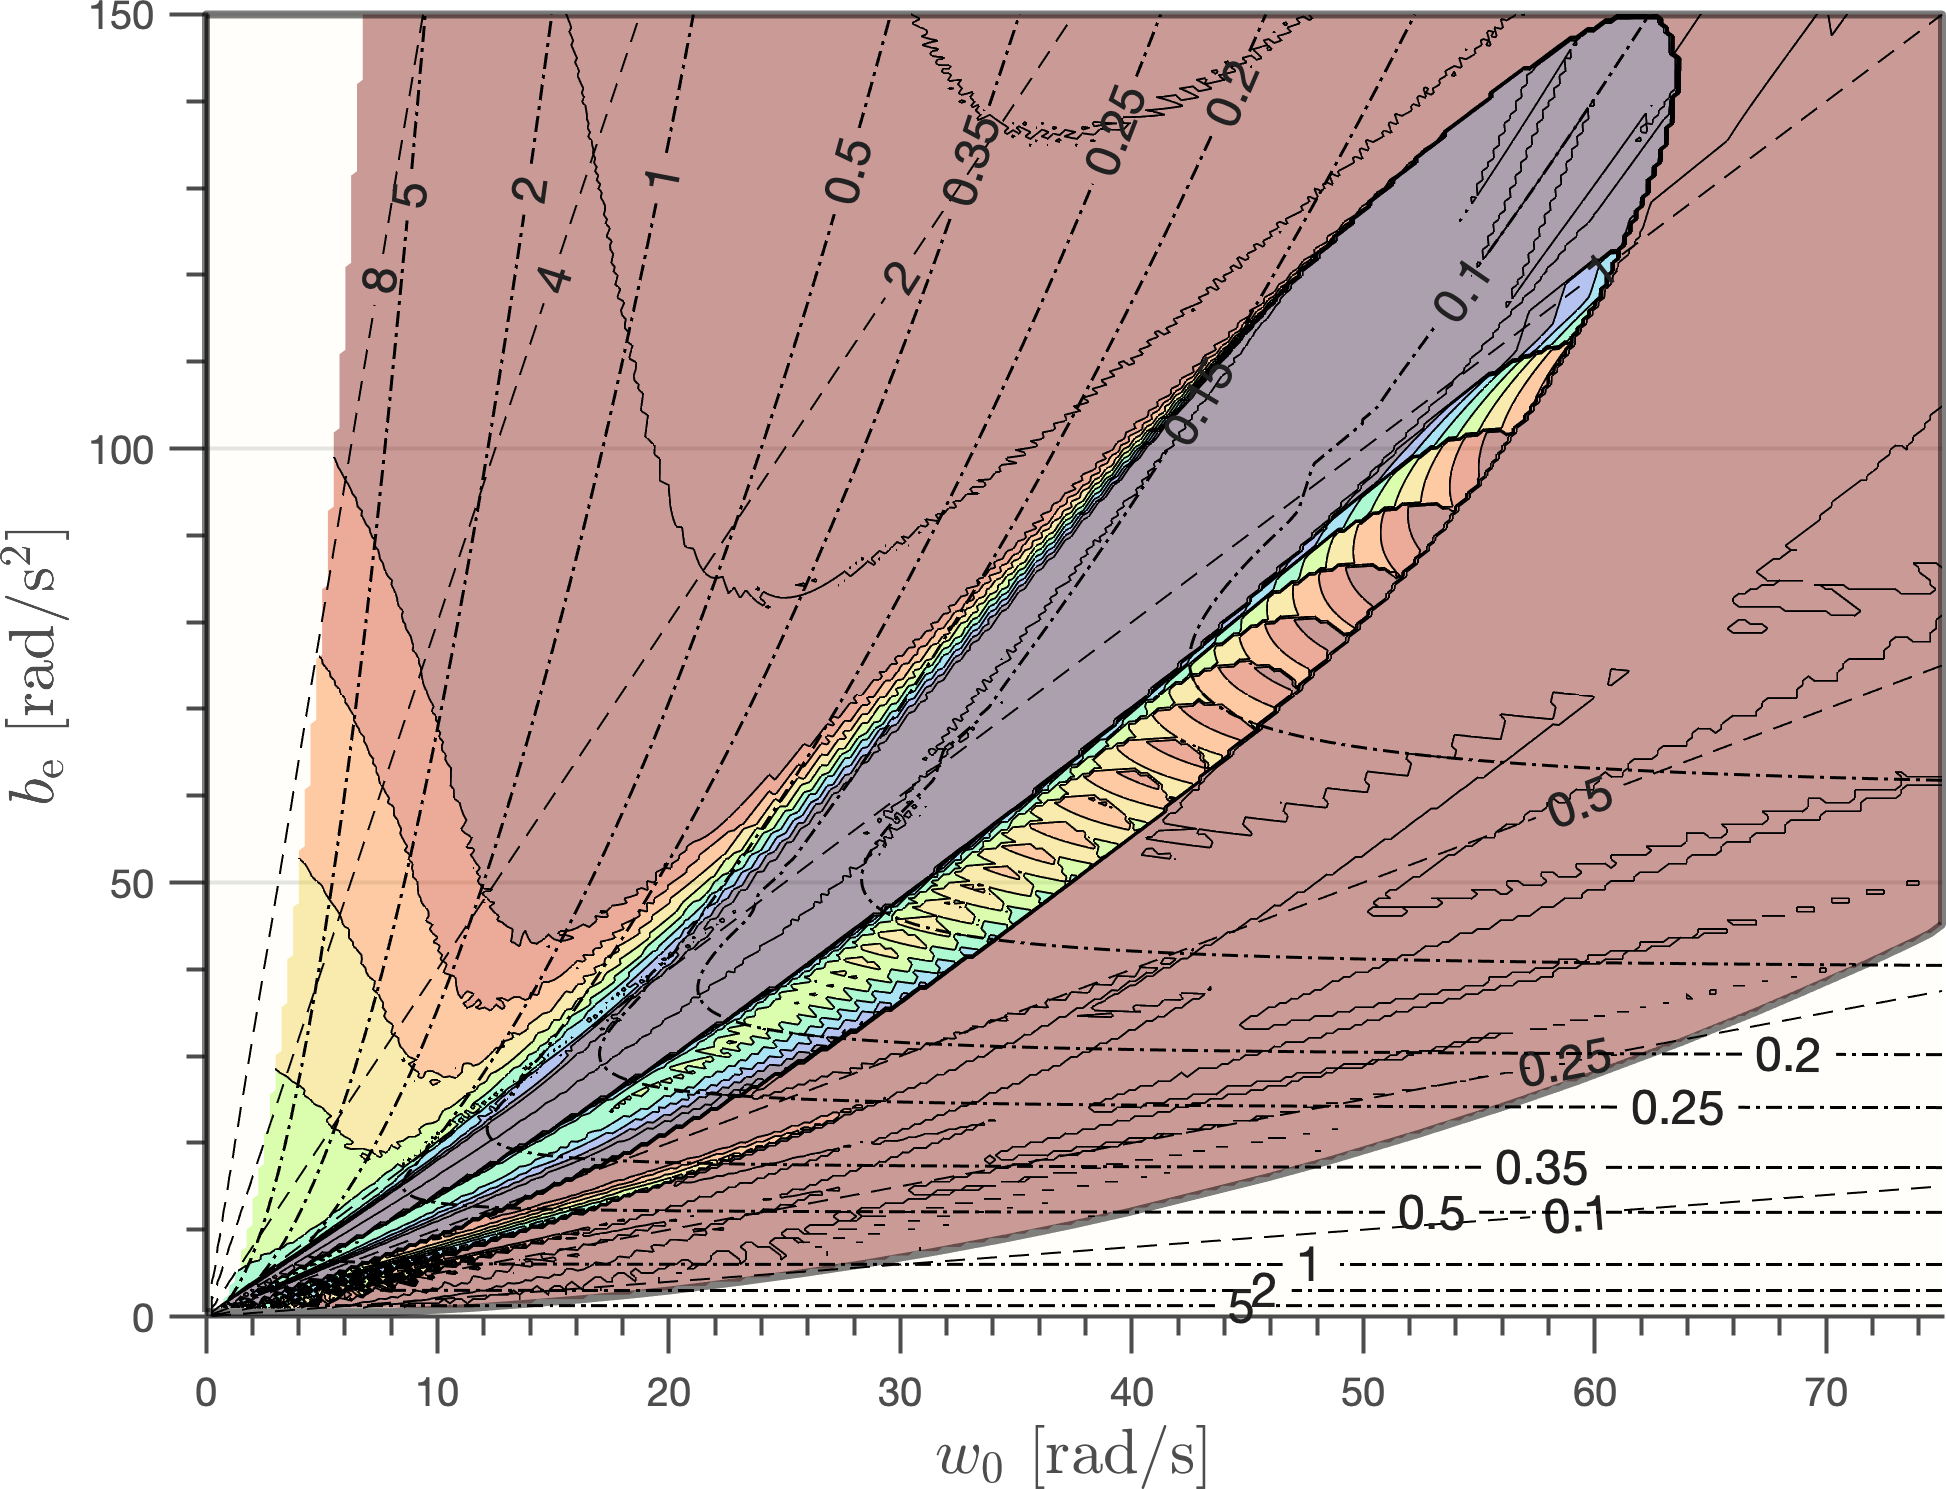
\includegraphics[width=\textwidth]{images/stab_map_0005.png}
    \caption{Stabilitástérkép 5ms időkéséssel}\label{fig:stab_map_0005}
    \end{center}
\end{figure}

\begin{figure}[H]
    \begin{center}
    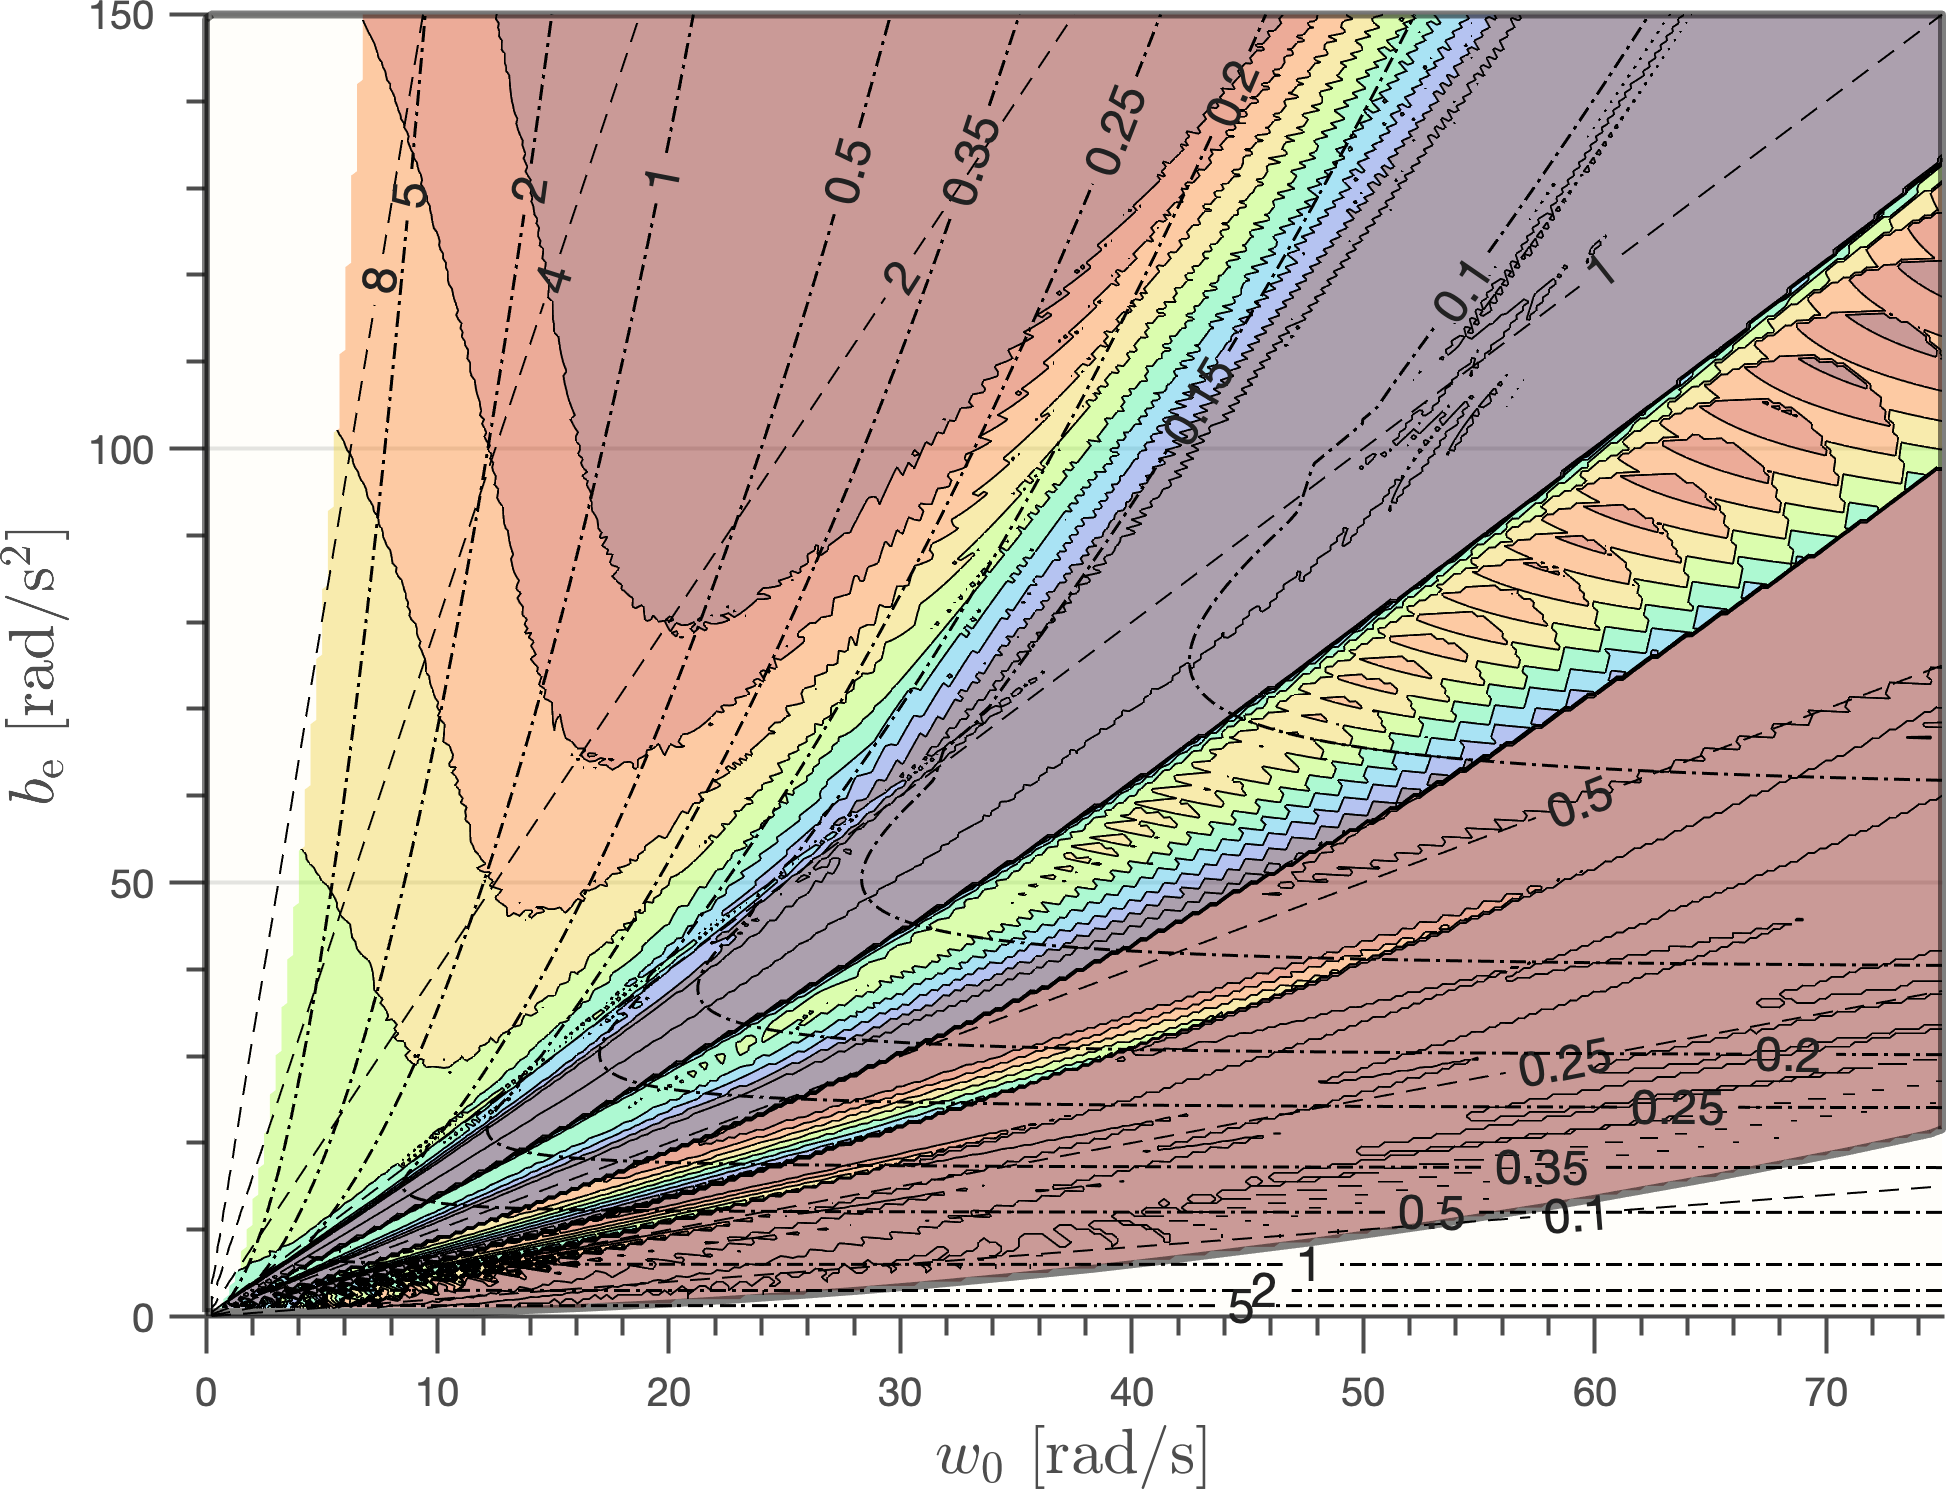
\includegraphics[width=\textwidth]{images/stab_map_00025.png}
    \caption{Stabilitástérkép 2.5ms időkéséssel}\label{fig:stab_map_00025}
    \end{center}
\end{figure}

\begin{figure}[H]
    \begin{center}
    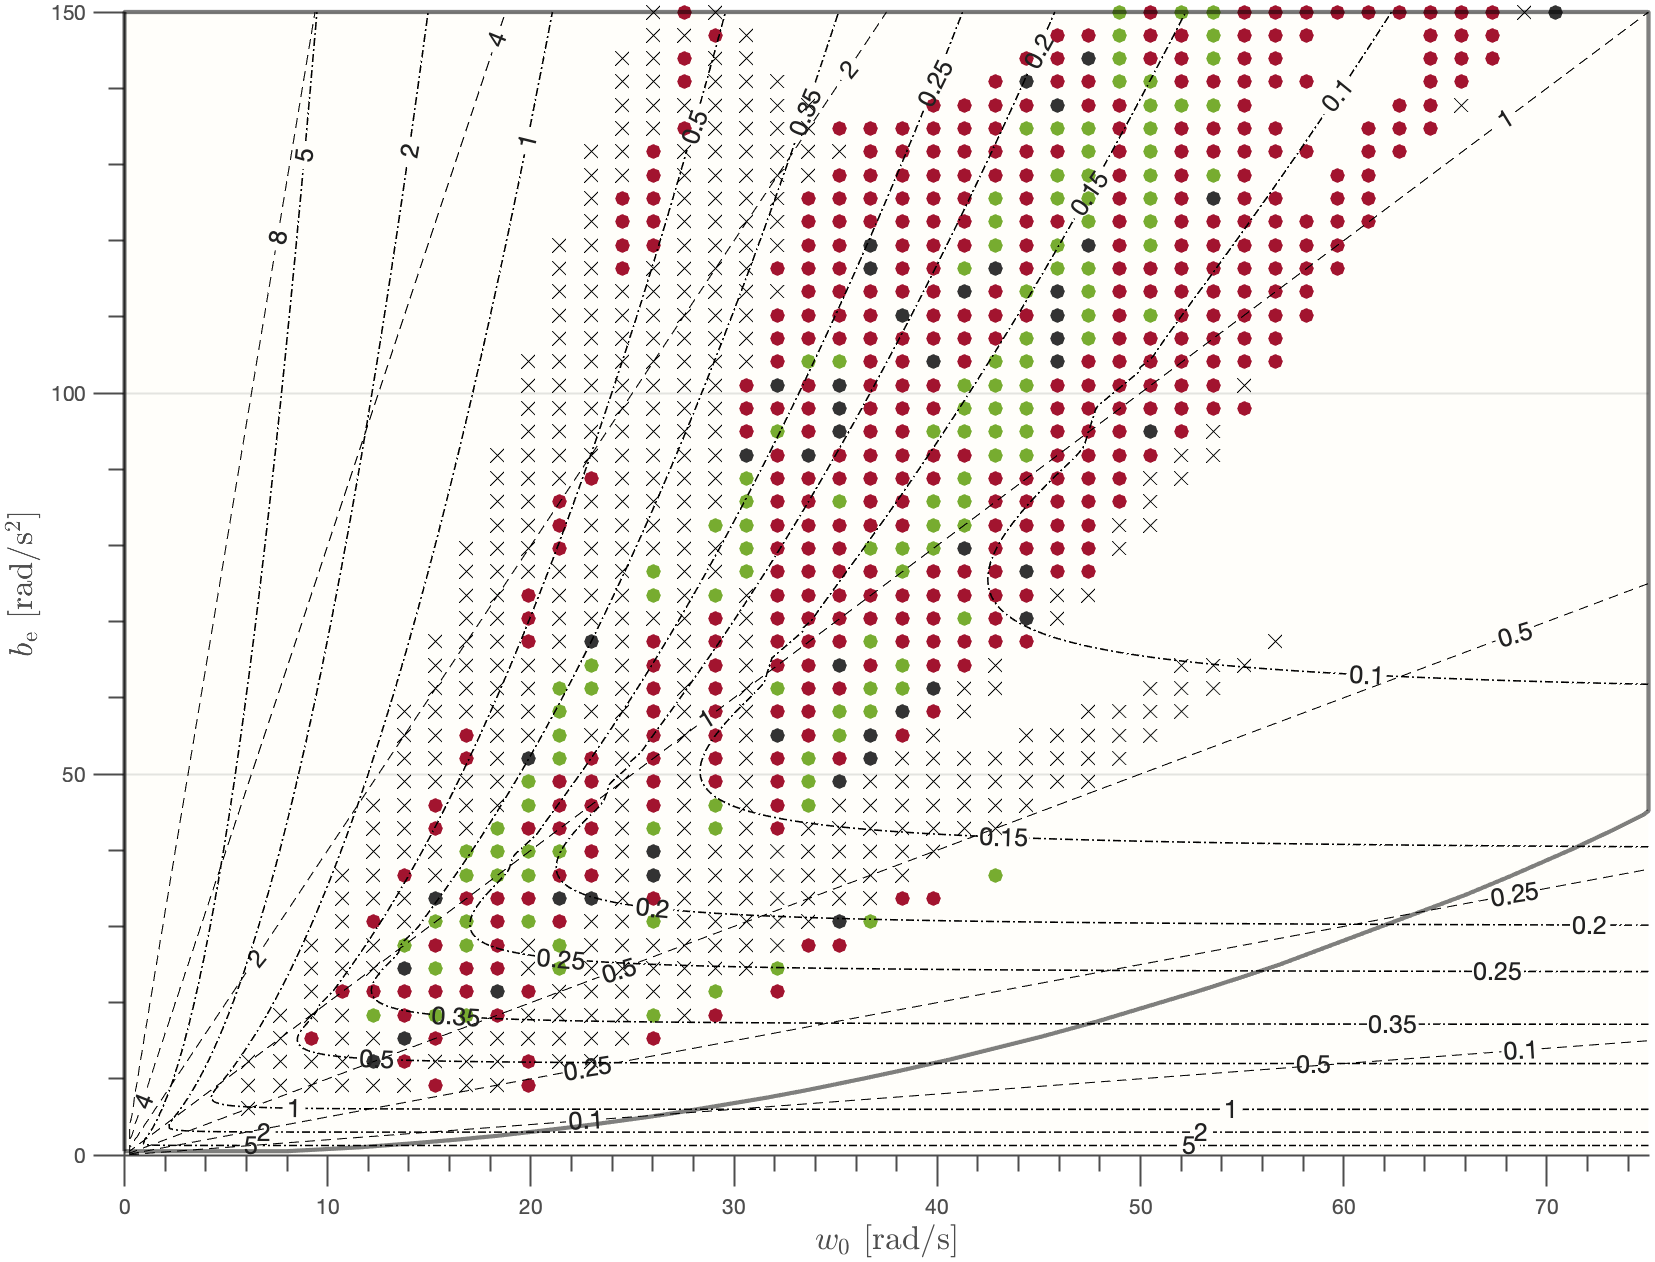
\includegraphics[width=\textwidth]{images/experiment_comparison_0005.png}
    \caption{Mért beállási idők összehasonlítása a modellel 5ms késéssel}\label{fig:experiment_comparison_0005}
    \end{center}
\end{figure}